\section[Pointer Swizzling in the DBMS Buffer Management]{Pointer Swizzling as in ``In-Memory Performance for Big Data''} \label{sec:paper}

\frame{\sectionpage}

\begin{frame}

	\frametitle{Five Layer Architecture of a DBMS \large(\cite{Haerder:1983} \cite{Haerder:1985})}
	
	\begin{columns}
      		\column{.5\textwidth}
		
			\tikzset{%
				every node/.style = {font = \sffamily},
				layer/.style = {rectangle, draw, thick},
				application/.style = {layer},
				datastructures/.style = {layer},
				accesspaths/.style = {layer},
				storagestructures/.style = {layer},
				propagationcontrol/.style = {layer},
				fileservices/.style = {layer},
				disk/.style = {cylinder, cylinder uses custom fill, shape border rotate = 90, draw, minimum height = 1cm, minimum width = 4cm, thick},
				disktext/.style = {},
				interfacearrow/.style = {<->, thick, draw = black},
				application/.append style = {color = Black, fill = Black!15},
				datastructures/.append style = {color = YellowOrange, fill = YellowOrange!15},
				accesspaths/.append style = {color = RedOrange, fill = RedOrange!15},
				storagestructures/.append style = {color = Red, fill = Red!15},
				propagationcontrol/.append style = {color = BrickRed, fill = BrickRed!15},
				fileservices/.append style = {color = Purple, fill = Purple!15},
				disk/.append style = {color = Blue, cylinder body fill = Blue!15, cylinder end fill = Blue!40},
				disktext/.append style = {color = Blue}
			}

			\centering
			\begin{adjustbox}{totalheight = \textheight - 4.0em}
				\begin{tikzpicture}[node distance = 5ex]
					\node[visible on = <9->, application]							(tp)			[]				{Transaction Programs};
					\node[visible on = <7->, datastructures]						(lgs)			[below = of tp]		{Logical Data Structures};
					\node[visible on = <6->, accesspaths]						(lap)			[below = of lgs]		{Logical Access Paths};
					\node[visible on = <5->, storagestructures]					(ss)			[below = of lap]		{Storage Structures};
					\node[visible on = <2->, propagationcontrol]					(pc)			[below = of ss]		{Propagation Control};
					\node[visible on = <3->, fileservices]							(fs)			[below = of pc]		{File Services\vphantom{g}};
							
					\node[visible on = <4->, disk]								(storage)		[below = of fs]		{};
			
					\node at (storage)	[visible on = <4->, disktext]				(storaget)		[]				{\small Secondary Storage};

					\path[visible on = <7->, interfacearrow]		(tp)		--	node[left]	{Set-Oriented Interface}		node[right]	{\emph{SQL, QBE}}													(lgs);
					\path[visible on = <6->, interfacearrow]		(lgs)		--	node[left]	{Record-Oriented Interface}	node[right]	{\small \lstinline|next()|\emph{, }\lstinline|remove()|\emph{, }\lstinline|add()| record}	(lap);
					\path[visible on = <5->, interfacearrow]		(lap)		--	node[left]	{Internal Record Interface}		node[right]	{\emph{store record in index}}											(ss);
					\path[visible on = <2->, interfacearrow]		(ss)		--	node[left]	{Buffer Interface}			node[right]	{\small \lstinline|fix()|\emph{, }\lstinline|unfix()|\emph{, }\lstinline|refix()|\emph{ page}}	(pc);
					\path[visible on = <3->, interfacearrow]		(pc)		--	node[left]	{File Interface}				node[right]	{\small \lstinline|fread()|\emph{, }\lstinline|fwrite()|\emph{ block}}					(fs);
					\path[visible on = <4->, interfacearrow]		(fs)		--	node[left]	{Device Interface}			node[right]	{\emph{channel programs}}											(storage);
				\end{tikzpicture}
			\end{adjustbox}
		
		\column{.5\textwidth}
			\only<2-9>{\begin{itemize}
				\only<2-2>{\item	Mainly consists of the \emph{DBMS buffer bool}}
				\only<2-2>{\item	Pages can be fixed and unfixed by upper layers}
				\only<2-2>{\item	Offers copies of persistent data in main memory}
				\only<3-3>{\item	Also called \emph{file management}}
				\only<3-3>{\item	Offers dynamically growing files and blocks of different length}
				\only<3-3>{\item	Manages file addresses, block borders and unused space}
				\only<3-3>{\item	Abstracts from the different characteristics of \emph{secondary storage devices}}
				\only<4-4>{\item	HDDs, SSDs etc.}
				\only<4-4>{\item	Interface is partially device specific}
				\only<5-5>{\item	Also called \emph{record and access path management}}
				\only<5-5>{\item	B* trees, hash indexes etc.}
				\only<5-5>{\item	Allows to navigate through those storage structures}
				\only<5-5>{\item	Maps records to pages}
				\only<5-5>{\item	Commonly offers variable-sized fields, large fields and references between records}
				\only<6-6>{\item	Also called \emph{navigational access layer}}
				\only<6-6>{\item	Offers an iterator interface over the resulting records}
				\only<6-6>{\item	Allows sorting and selection but no more complex operations}
				\only<6-6>{\item	Introduces data types}
				\only<6-6>{\item	Uppermost interface of \emph{navigational} or \emph{hierarchical databases}}
				\only<7-7>{\item	Also called \emph{non-procedural access layer}}
				\only<7-7>{\item	Offers complex descriptive query languages like \emph{SQL}, \emph{QBE} or \emph{XQuery}}
				\only<7-7>{\item	Maps external identifiers of e.g. relations, views and tuples to internal identifiers using the \emph{metadata management}}
				\only<8-8>{\item	Offers complex set operations}
				\only<8-8>{\item	Offers \emph{data integrity}, \emph{access control} and \emph{transaction managment}}
				\only<8-8>{\item	Most interesting target for the \emph{query optimizer}}
				\only<9-9>{\item	Application programs uses the service of the DBMS to store persistent data}
			\end{itemize}}
				
	\end{columns}

\end{frame}

\begin{frame}

	\frametitle{Motivation for the Usage of a Buffer Pool (1)}
	
	\tikzset{%
		changes/.style = { -> , very thick, > = stealth},
		volatile/.style = {fill = red!50},
		nonvolatile/.style = {fill = green!50},
		changes/.append style = {color = red}
	}

	\centering
	\noindent\makebox[\textwidth]{
		\begin{adjustbox}{width = \textwidth + 4.0em}
			\begin{tikzpicture}[]
						% Center points of the baseline of each pyramid layer (0: Peak of the pyramid; 1: Center of the baseline of the top layer; ...)
						\node[]			(0)															{};
						\node[]			(1)		[below = 1.2*1.5cm of 0.center, anchor = center]					{};
						\node[]			(2a)		[below = 1.2*(1/3)*1.25cm of 1.center, anchor = center]				{};
						\node[]			(2b)		[below = 1.2*(1/3)*1.25cm of 2a.center, anchor = center]				{};
						\node[]			(2c)		[below = 1.2*(1/3)*1.25cm of 2b.center, anchor = center]				{};
						\node[]			(3)		[below = 1.2*0.75cm of 2c.center, anchor = center]					{};
						\node[]			(4)		[below = 1.2*0.75cm of 3.center, anchor = center]					{};
						\node[]			(5)		[below = 1.2*0.75cm of 4.center, anchor = center]					{};
						\node[]			(6)		[below = 1.2*0.75cm of 5.center, anchor = center]					{};

						% Anchor points of the pyramid (n0: Left anchor point; n1: Right anchor point):
						\node[]			(10)		[left = (2/3)*1.5cm of 1.center, anchor = center]					{};
						\node[]			(11)		[right = (2/3)*1.5cm of 1.center, anchor = center]				{};
						\node[]			(2a0)		[left = (2/3)*(1.5cm+(1/3)*1.25cm) of 2a.center, anchor = center]	{};
						\node[]			(2a1)		[right = (2/3)*(1.5cm+(1/3)*1.25cm) of 2a.center, anchor = center]	{};
						\node[]			(2b0)		[left = (2/3)*(1.5cm+(2/3)*1.25cm) of 2b.center, anchor = center]	{};
						\node[]			(2b1)		[right = (2/3)*(1.5cm+(2/3)*1.25cm) of 2b.center, anchor = center]	{};
						\node[]			(2c0)		[left = (2/3)*(1.5cm+(3/3)*1.25cm) of 2c.center, anchor = center]	{};
						\node[]			(2c1)		[right = (2/3)*(1.5cm+(3/3)*1.25cm) of 2c.center, anchor = center]	{};
						\node[]			(30)		[left = (2/3)*3.5cm of 3.center, anchor = center]					{};
						\node[]			(31)		[right = (2/3)*3.5cm of 3.center, anchor = center]				{};
						\node[]			(40)		[left = (2/3)*4.25cm of 4.center, anchor = center]				{};
						\node[]			(41)		[right = (2/3)*4.25cm of 4.center, anchor = center]				{};
						\node[]			(50)		[left = (2/3)*5cm of 5.center, anchor = center]					{};
						\node[]			(51)		[right = (2/3)*5cm of 5.center, anchor = center]					{};
						\node[]			(60)		[left = (2/3)*5.75cm of 6.center, anchor = center]				{};
						\node[]			(61)		[right = (2/3)*5.75cm of 6.center, anchor = center]				{};
		
						% "Center" of the pyramid (shifted towards top) used for the designation of performance measures:
						\node[]			(cen)		[below = 2.5cm of 0.center]								{};
		
						% Designation of performance measures:
						\node[visible on = <2->, rotate = 61]	(cpu)		[left = 3.25cm of cen.center, anchor = center]				{\footnotesize \textit{\textbf{Capacity per CPU}}};
						\node[visible on = <2->, rotate = -61]	(acc)		[right = 4.25cm of cen.center, anchor = center]				{\footnotesize \textit{\textbf{Access Time}}};
		
						% Fills the pyramid to mark volatile and non-volatile layers:
						\fill[visible on = <9->, volatile]
							(0.center) -- (30.center) -- (31.center) -- cycle;
						\fill[visible on = <9->, nonvolatile]
							(30.center) -- (31.center) -- (61.center) -- (60.center) -- cycle;
		
						% Key the markings for volatile and non-volatile layers
						\node[visible on = <9->, draw, volatile]		(red)		[left = 4cm of 0.center, anchor = north]		{};
						\node[visible on = <9->]					(legred)	[right = 0cm of red.east, anchor = west]		{\footnotesize Volatile};
						\node[visible on = <9->, draw, nonvolatile]		(green)	[below = 0.2cm of red.south, anchor = north]	{};
						\node[visible on = <9->]					(leggreen)	[right = 0cm of green.east, anchor = west]		{\footnotesize Non-volatile};

						% Storage layer names:
						\node[visible on = <2->]	(reg)		[above = 0cm of 1.center, anchor = south]		{\footnotesize Registers};
						\node[visible on = <3->]	(l1)		[above = 0cm of 2a.center, anchor = south]	{\footnotesize L1 Cache};
						\node[visible on = <3->]	(l2)		[above = 0cm of 2b.center, anchor = south]	{\footnotesize L2 Cache};
						\node[visible on = <3->]	(l3)		[above = 0cm of 2c.center, anchor = south]	{\footnotesize L3 Cache};
						\node[visible on = <4->]	(mem)	[above = 0.05cm of 3.center, anchor = south]	{\small Main Memory};
						\node[visible on = <5->]	(ssd)		[above = 0.05cm of 4.center, anchor = south]	{\small Online Storage \scriptsize \textit{(Secondary S.) - SDD}};
						\node[visible on = <6->]	(mas)	[above = 0.05cm of 5.center, anchor = south]	{\small Online Storage \scriptsize \textit{(Secondary S.) - HDD}};
						\node[visible on = <7->]	(mem)	[above = 0.05cm of 6.center, anchor = south]	{\small Offline Storage \scriptsize \textit{(Tertiary Storage)}};

						% Anchor points for the brace used to mark the example data from Intel Xeon:
						\node[]	(0h)		[right = 2.75cm of 0]		{};
						\node[]	(31h)		[right = 2.75cm of 31]	{};
		
						% Draw the pyramid:
						\path[ - , thick]
							(0.center)			edge	[visible on = <1->]	(10.center)
							(0.center)			edge[visible on = <1->]	(11.center)
							(10.center)		edge[visible on = <2->]	(11.center)
							(10.center)		edge	[visible on = <1->]	(2a0.center)
							(11.center)		edge	[visible on = <1->]	(2a1.center)
							(2a0.center)		edge	[visible on = <3->]	(2a1.center)
							(2a0.center)		edge	[visible on = <1->]	(2b0.center)
							(2a1.center)		edge[visible on = <1->]	(2b1.center)
							(2b0.center)		edge[visible on = <3->]	(2b1.center)
							(2b0.center)		edge[visible on = <1->]	(2c0.center)
							(2b1.center)		edge[visible on = <1->]	(2c1.center)
							(2c0.center)		edge[visible on = <3->]	(2c1.center)
							(2c0.center)		edge[visible on = <1->]	(30.center)
							(2c1.center)		edge[visible on = <1->]	(31.center)
							(30.center)		edge[visible on = <4->]	(31.center)
							(30.center)		edge[visible on = <1->]	(40.center)
							(31.center)		edge	[visible on = <1->]	(41.center)
							(40.center)		edge	[visible on = <5->]	(41.center)
							(40.center)		edge[visible on = <1->]	(50.center)
							(41.center)		edge	[visible on = <1->]	(51.center)
							(50.center)		edge	[visible on = <6->]	(51.center)
							(50.center)		edge	[visible on = <1->]	(60.center)
							(51.center)		edge[visible on = <1->]	(61.center)
							(60.center)		edge	[visible on = <1->]	(61.center);
		
						% Draw the connections between the brace used to mark the example data from Intel Xeon and the appropriate pyramid layers:
						\path[visible on = <4->, dotted]
							(0.center)				edge		(0h.center)
							(31.center)			edge		(31h.center);
			
						% Add the capacities:
						\draw [visible on = <2->, decorate, decoration = {brace, mirror, amplitude = 3.75pt}]
							(0.center) -- (10.center) node[black, midway, xshift = -0.1cm, yshift = 0.1cm, anchor = east] {\SI{128}{\byte}};
						\draw [visible on = <3->, decorate, decoration = {brace, mirror, amplitude = 3.75pt}]
							(10.center) -- (2a0.center) node[black, midway, xshift = -0.1cm, yshift = 0.1cm, anchor = east] {\small \SI{256}{\kibi\byte}};
						\draw [visible on = <3->, decorate, decoration = {brace, mirror, amplitude = 3.75pt}]
							(2a0.center) -- (2b0.center) node[black, midway, xshift = -0.1cm, yshift = 0.1cm, anchor = east] {\small \SI{1}{\mebi\byte}};
						\draw [visible on = <3->, decorate, decoration = {brace, mirror, amplitude = 3.75pt}]
							(2b0.center) -- (2c0.center) node[black, midway, xshift = -0.1cm, yshift = 0.1cm, anchor = east] {\small \SI{8}{\mebi\byte}};
						\draw [visible on = <4->, decorate, decoration = {brace, mirror, amplitude = 3.75pt}]
							(2c0.center) -- (30.center) node[black, midway, xshift = -0.1cm, yshift = 0.1cm, anchor = east] {\SI{64}{\gibi\byte}};
						\draw [visible on = <5->, decorate, decoration = {brace, mirror, amplitude = 3.75pt}]
							(30.center) -- (40.center) node[black, midway, xshift = -0.1cm, yshift = 0.1cm, anchor = east] {\si{\tebi\byte}};
						\draw [visible on = <6->, decorate, decoration = {brace, mirror, amplitude = 3.75pt}]
							(40.center) -- (50.center) node[black, midway, xshift = -0.1cm, yshift = 0.1cm, anchor = east] {\si{\tebi\byte}--\si{\pebi\byte}};
						\draw [visible on = <7->, decorate, decoration = {brace, mirror, amplitude = 3.75pt}]
							(50.center) -- (60.center) node[black, midway, xshift = -0.1cm, yshift = 0.1cm, anchor = east] {\si{\pebi\byte}};

						% Add the access times:
						\draw [visible on = <2->, decorate, decoration = {brace, amplitude = 3.75pt}]
							(0.center) -- (11.center) node[black, midway, xshift = 0.1cm, yshift = 0.1cm, anchor = west] {\SI{1}{\cy} $\approx$ \SI{0.25}{\nano\second}};
						\draw [visible on = <3->, decorate, decoration = {brace, amplitude = 3.75pt}]
							(11.center) -- (2a1.center) node[black, midway, xshift = 0.1cm, yshift = 0.1cm, anchor = west] {\small \SI{4}{\cy} $\approx$ \SI{1}{\nano\second}};
						\draw [visible on = <3->, decorate, decoration = {brace, amplitude = 3.75pt}]
							(2a1.center) -- (2b1.center) node[black, midway, xshift = 0.1cm, yshift = 0.1cm, anchor = west] {\small \SI{12}{\cy} $\approx$ \SI{3}{\nano\second}};
						\draw [visible on = <3->, decorate, decoration = {brace, amplitude = 3.75pt}]
							(2b1.center) -- (2c1.center) node[black, midway, xshift = 0.1cm, yshift = 0.1cm, anchor = west] {\small \SI{42}{\cy} $\approx$ \SI{11}{\nano\second}};
						\draw [visible on = <4->, decorate, decoration = {brace, amplitude = 3.75pt}]
							(2c1.center) -- (31.center) node[black, midway, xshift = 0.1cm, yshift = 0.1cm, anchor = west] {\SI{51}{\nano\second}};
						\draw [visible on = <5->, decorate, decoration = {brace, amplitude = 3.75pt}]
							(31.center) -- (41.center) node[black, midway, xshift = 0.1cm, yshift = 0.1cm, anchor = west] {\SI{\approx 0.1}{\milli\second} \tiny \cite{samsung:ssdprimer}};
						\draw [visible on = <6->, decorate, decoration = {brace, amplitude = 3.75pt}]
							(41.center) -- (51.center) node[black, midway, xshift = 0.1cm, yshift = 0.1cm, anchor = west] {\numrange{5}{20}\si{\milli\second} \tiny \cite{EntHDD} \cite{HDD2016}};
						\draw [visible on = <7->, decorate, decoration = {brace, amplitude = 3.75pt}]
							(51.center) -- (61.center) node[black, midway, xshift = 0.1cm, yshift = 0.1cm, anchor = west] {$s - min$};

						% Mark the source of the performance data of the volatile layers:
						\draw [visible on = <4->, decorate, decoration = {brace, amplitude = 3.75pt}]
							(0h.center) -- (31h.center) node[black, midway, xshift = -0.625cm, yshift = 0.1cm, anchor = west] {\footnotesize \begin{tabular}{r}\textit{\textbf{Example System:}}\\\textit{Intel\textsuperscript{\tiny\textregistered} Xeon\textsuperscript{\tiny\textregistered}}\\\textit{E3-1280 v5}\\\textit{(Skylake)}\\\cite{7cpu:skylake}\end{tabular}};
			
						% Orientation of changes of performance data:
						\path[visible on = <8->, changes]
							([xshift = (-1/3)*4cm+0.25cm]60.center)			edge		node[above, rotate = 90]		{\footnotesize Price per Capacity}	([xshift = (-1/3)*14cm-0.25cm]0.center)
							([xshift = (1/3)*18cm+0.5cm]0.center)			edge		node[above, rotate = -90]		{\footnotesize Access Time}		([xshift = (1/3)*8cm]61.center);
			\end{tikzpicture}
		\end{adjustbox}
	}

\end{frame}

\begin{frame}

	\frametitle{Motivation for the Usage of a Buffer Pool (2)}

	\begin{block}{\uncover<2->{Requirements of Memory for a DBMS}}
		\begin{itemize}
			\uncover<3->{\item	\textbf{Low latency}}\uncover<4->{\textbf{: }Main memory}
			\uncover<5->{\item	\textbf{High capacity}}\uncover<6->{\textbf{: }Secondary Storage}
			\uncover<7->{\item	\textbf{Non-volatility}}\uncover<8->{\textbf{: }Secondary Storage}
			\uncover<9->{\item	\textbf{Byte-addressable}}\uncover<10->{\textbf{: }Main memory}
		\end{itemize}
	\end{block}
	
	\uncover<11->{$\implies$ \textbf{Caching:} Persistently store the database on \emph{secondary storage} and cache a subset of it in \emph{main memory}.}

\end{frame}

\subsection{Some Tasks of the DBMS Buffer Management}

\frame{\subsectionpage}

\begin{frame}

	\frametitle{Memory Allocation in the Buffer Pool \large(\cite{Datenbanksysteme_-_Konzepte_und_Techniken_der_Implementierung})}

	\tikzset{%
		every node/.style = {rectangle, draw = black, very thick, rounded corners, font = \Large}, 
		level 1/.style={level distance = 2.5cm, sibling distance = 3cm}, 
		level 2/.style={level distance = 2.5cm, sibling distance = 2cm}, 
		level 3/.style={level distance = 2.5cm, sibling distance = 4.5cm}, 
		edge from parent/.style = {draw = black, very thick},
		every node/.append style = {draw = black, fill = black!15, text = black}, 
		edge from parent/.append style = {draw = black}
	}

	\centering
	\begin{adjustbox}{totalheight = \textheight - 4.0em}
		\begin{tikzpicture}[]
			\node[visible on = <2->]								(algorithms)		[]		{\textbf{Allocation Strategy}}
				child[visible on = <8->] {node[]						(global)			[]		{global}}
				child[visible on = <3->] {node[]						(local)			[]		{local/ partitioned}
					child[visible on = <7->] {node[]					(dynamic)			[]		{dynamic}}
 					child[visible on = <4->] {node[]					(static)			[]		{static\vphantom{y}}
						child[visible on = <5->] {node[]				(uniform)			[]		{uniform partitions}}
						child[visible on = <6->] {node[]				(adjusted)			[]		{adjusted partitions}}}
			};
			
		\end{tikzpicture}
	\end{adjustbox}

\end{frame}

\begin{frame}

	\frametitle{Concurrency Control}

	\begin{itemize}
		\uncover<2->{\item	\textbf{Pages} get accessed concurrently}
			\begin{itemize}
				\uncover<3->{\item	Latching for the pages}
				\uncover<4->{\item	Mutually exclusive write accesses}
				\uncover<5->{\item	Concurrent read accesses}
			\end{itemize}
		\uncover<6->{\item	\textbf{Auxiliary data} gets accessed concurrently}
			\begin{itemize}
				\uncover<7->{\item	Latching for the auxiliary data structures}
				\uncover<8->{\item	... or the usage of special concurrent implementations of the data structures}
			\end{itemize}
	\end{itemize}

\end{frame}

\subsection{Locate Pages in the Buffer Pool without Pointer Swizzling}

\frame{\subsectionpage}

\begin{frame}

	\frametitle{Overview of Search Strategies \large(\cite{Datenbanksysteme_-_Konzepte_und_Techniken_der_Implementierung})}

	\tikzset{%
		every node/.style = {rectangle, draw = black, inner xsep = -0.75mm, very thick, rounded corners}, 
		level 1/.style={level distance = 3cm, sibling distance = 4cm}, 
		level 2/.style={level distance = 3cm, sibling distance = 2cm}, 
		edge from parent/.style = {draw = black, very thick},
		every node/.append style = {draw = black, fill = black!15, text = black}, 
		edge from parent/.append style = {draw = black}
	}

	\centering
	\begin{adjustbox}{width = \textwidth}
		\begin{tikzpicture}
			\node[visible on = <2->]								(algorithms)		[]		{\begin{tabular}{c}Search\\Strategy\end{tabular}}
				child[visible on = <3->] {node[]						(seq)				[]		{\begin{tabular}{c}Direct Search in\\the Buffer Frames\end{tabular}}}
				child[visible on = <4->] {node[]						(aux)				[]		{\begin{tabular}{c}Indirect Search Using\\Auxiliary Tables\end{tabular}}
					child[visible on = <5->] {node[]					(trans)			[]		{\begin{tabular}{c}Translation\\Table\end{tabular}}}
 					child[visible on = <6->] {node[]					(unsort)			[]		{\begin{tabular}{c}Unsorted\\Table\end{tabular}}}
 					child[visible on = <7->] {node[]					(sort)				[]		{\begin{tabular}{c}Sorted\\Table\end{tabular}}}
					child[visible on = <8->] {node[]					(chain)			[]		{\begin{tabular}{c}Chained\\Table\end{tabular}}}
					child[visible on = <9->] {node[]					(tree)			[]		{\begin{tabular}{c}Search\\Trees\end{tabular}}}
					child[visible on = <10->] {node[]					(hash)			[]		{\begin{tabular}{c}Hash\\Table\end{tabular}}}
			};
		
		\end{tikzpicture}
	\end{adjustbox}

\end{frame}

\begin{frame}

	\frametitle{Direct Search in the Buffer Frames \& Unsorted Table}
	
	\begin{block}{\uncover<2->{Direct Search in the Buffer Frames}}
		\begin{itemize}
			\uncover<3->{\item	Checks in each buffer frame the page ID of the contained page}
			\uncover<4->{\item	$T_{\text{avg}}^{\text{search}} \in \mathcal O\left(\frac{n}{2}\right)$, $T_{\text{worst}}^{\text{search}} \in  \mathcal O\left(n\right)$}
			\uncover<5->{\item	The usage of virtual memory management can result in extensive swapping due to read access to many pages!}
		\end{itemize}
	\end{block}

	\begin{block}{\uncover<6->{Unsorted Table}}
		\begin{itemize}
			\uncover<7->{\item	Auxiliary data structure of size $S\text{\tiny{pace}} \in \mathcal O\left(n\right)$}
			\uncover<8->{\item	$T_{\text{avg}}^{\text{search}} \in \mathcal O\left(\frac{n}{2}\right)$, $T_{\text{worst}}^{\text{search}} \in  \mathcal O\left(n\right)$}
		\end{itemize}
	\end{block}

	\tikzset{%
		table/.style = {draw = black, shape = rectangle split, rectangle split parts = 9, rectangle split horizontal, font = \bfseries}
	}

	\centering
	\vspace{-1.0em}
	\uncover<7->{\begin{figure}[ht!]
		\begin{adjustbox}{width = \textwidth}
			\begin{tikzpicture}
				\node[table]	(table)	{\nodepart{one}7785\nodepart{two}6977\nodepart{three}4347\nodepart{four}3380\nodepart{five}5610\nodepart{six}6376\nodepart{seven}4877\nodepart{eight}3332\nodepart{nine}3354};
				
				\foreach \anchor/\address in {one/0, two/1, three/2, four/3, five/4, six/5, seven/6, eight/7, nine/8} {
					\node[]	(\address)		[above = .375cm of table.\anchor]	{\address};
				}
			\end{tikzpicture}
		\end{adjustbox}
		\vspace{-2.0em}
		\caption{An unsorted table used to map buffer frames to page IDs.}
	\end{figure}}

\end{frame}

\begin{frame}

	\frametitle{Translation Table}
	
	\begin{itemize}
		\uncover<2->{\item	Auxiliary data structure with one entry per page in the database $\implies S\text{\tiny{pace}} \in \mathcal O\left(p\right)$}
		\uncover<3->{\item	$T^{\text{search}} \in  \mathcal O\left(1\right)$, $T^{\text{insert}} \in  \mathcal O\left(1\right)$}
	\end{itemize}

	\centering
	\uncover<2->{\begin{figure}[ht!]
		\begin{adjustbox}{width = \textwidth}
			\begin{tabular}{cc}
																		\hline
				\multicolumn{1}{|c|}{0}		& \multicolumn{1}{c|}{$\cdot$} 		\\ 	\hline
				\multicolumn{2}{c}{$\vdots$}                                   		\\ 	\hline
				\multicolumn{1}{|c|}{3331}		& \multicolumn{1}{c|}{$\cdot$} 		\\ 	\hline
				\multicolumn{1}{|c|}{3332}		& \multicolumn{1}{c|}{7}       		\\ 	\hline
				\multicolumn{1}{|c|}{3333}		& \multicolumn{1}{c|}{$\cdot$} 		\\ 	\hline
				\multicolumn{2}{c}{$\vdots$}                                  
			\end{tabular}
			\begin{tabular}{cc}
				\multicolumn{2}{c}{$\vdots$}                                   		\\ 	\hline
				\multicolumn{1}{|c|}{3352}		& \multicolumn{1}{c|}{$\cdot$} 		\\ 	\hline
				\multicolumn{1}{|c|}{3353}		& \multicolumn{1}{c|}{$\cdot$} 		\\ 	\hline
				\multicolumn{1}{|c|}{3354}		& \multicolumn{1}{c|}{8}       		\\ 	\hline
				\multicolumn{1}{|c|}{3355}		& \multicolumn{1}{c|}{$\cdot$} 		\\ 	\hline
				\multicolumn{1}{|c|}{3356}		& \multicolumn{1}{c|}{$\cdot$} 		\\ 	\hline
				\multicolumn{2}{c}{$\vdots$}                                  
			\end{tabular}
			\begin{tabular}{cc}
				\multicolumn{2}{c}{$\vdots$}                                   		\\ 	\hline
				\multicolumn{1}{|c|}{3378}		& \multicolumn{1}{c|}{$\cdot$} 		\\ 	\hline
				\multicolumn{1}{|c|}{3379}		& \multicolumn{1}{c|}{$\cdot$} 		\\ 	\hline
				\multicolumn{1}{|c|}{3380}		& \multicolumn{1}{c|}{3}       		\\ 	\hline
				\multicolumn{1}{|c|}{3381}		& \multicolumn{1}{c|}{$\cdot$} 		\\ 	\hline
				\multicolumn{1}{|c|}{3382}		& \multicolumn{1}{c|}{$\cdot$} 		\\ 	\hline
				\multicolumn{2}{c}{$\vdots$}                                  
			\end{tabular}
			\begin{tabular}{cc}
				\multicolumn{2}{c}{$\vdots$}                                   		\\ 	\hline
				\multicolumn{1}{|c|}{4345}		& \multicolumn{1}{c|}{$\cdot$} 		\\ 	\hline
				\multicolumn{1}{|c|}{4346}		& \multicolumn{1}{c|}{$\cdot$} 		\\ 	\hline
				\multicolumn{1}{|c|}{4347}		& \multicolumn{1}{c|}{2}       		\\ 	\hline
				\multicolumn{1}{|c|}{4348}		& \multicolumn{1}{c|}{$\cdot$} 		\\ 	\hline
				\multicolumn{1}{|c|}{4349}		& \multicolumn{1}{c|}{$\cdot$} 		\\ 	\hline
				\multicolumn{2}{c}{$\vdots$}                                  
			\end{tabular}
			\begin{tabular}{cc}
				\multicolumn{2}{c}{$\vdots$}                                   		\\ 	\hline
				\multicolumn{1}{|c|}{4875}		& \multicolumn{1}{c|}{$\cdot$} 		\\ 	\hline
				\multicolumn{1}{|c|}{4876}		& \multicolumn{1}{c|}{$\cdot$} 		\\ 	\hline
				\multicolumn{1}{|c|}{4877}		& \multicolumn{1}{c|}{6}       		\\ 	\hline
				\multicolumn{1}{|c|}{4878}		& \multicolumn{1}{c|}{$\cdot$} 		\\ 	\hline
				\multicolumn{1}{|c|}{4879}		& \multicolumn{1}{c|}{$\cdot$} 		\\ 	\hline
				\multicolumn{2}{c}{$\vdots$}                                  
			\end{tabular}
			\begin{tabular}{cc}
				\multicolumn{2}{c}{$\vdots$}                                   		\\ 	\hline
				\multicolumn{1}{|c|}{5608}		& \multicolumn{1}{c|}{$\cdot$} 		\\ 	\hline
				\multicolumn{1}{|c|}{5609}		& \multicolumn{1}{c|}{$\cdot$} 		\\ 	\hline
				\multicolumn{1}{|c|}{5610}		& \multicolumn{1}{c|}{4}       		\\ 	\hline
				\multicolumn{1}{|c|}{5611}		& \multicolumn{1}{c|}{$\cdot$} 		\\ 	\hline
				\multicolumn{1}{|c|}{5612}		& \multicolumn{1}{c|}{$\cdot$} 		\\ 	\hline
				\multicolumn{2}{c}{$\vdots$}                                  
			\end{tabular}
			\begin{tabular}{cc}
				\multicolumn{2}{c}{$\vdots$}                                   		\\ 	\hline
				\multicolumn{1}{|c|}{6374}		& \multicolumn{1}{c|}{$\cdot$} 		\\ 	\hline
				\multicolumn{1}{|c|}{6375}		& \multicolumn{1}{c|}{$\cdot$} 		\\ 	\hline
				\multicolumn{1}{|c|}{6376}		& \multicolumn{1}{c|}{5}       		\\ 	\hline
				\multicolumn{1}{|c|}{6377}		& \multicolumn{1}{c|}{$\cdot$} 		\\ 	\hline
				\multicolumn{1}{|c|}{6378}		& \multicolumn{1}{c|}{$\cdot$} 		\\ 	\hline
				\multicolumn{2}{c}{$\vdots$}                                  
			\end{tabular}
			\begin{tabular}{cc}
				\multicolumn{2}{c}{$\vdots$}                                   		\\ 	\hline
				\multicolumn{1}{|c|}{6975}		& \multicolumn{1}{c|}{$\cdot$} 		\\ 	\hline
				\multicolumn{1}{|c|}{6976}		& \multicolumn{1}{c|}{$\cdot$} 		\\ 	\hline
				\multicolumn{1}{|c|}{6977}		& \multicolumn{1}{c|}{1}       		\\ 	\hline
				\multicolumn{1}{|c|}{6978}		& \multicolumn{1}{c|}{$\cdot$} 		\\ 	\hline
				\multicolumn{1}{|c|}{6979}		& \multicolumn{1}{c|}{$\cdot$} 		\\ 	\hline
				\multicolumn{2}{c}{$\vdots$}                                  
			\end{tabular}
			\begin{tabular}{cc}
				\multicolumn{2}{c}{$\vdots$}                                   		\\ 	\hline
				\multicolumn{1}{|c|}{7783}		& \multicolumn{1}{c|}{$\cdot$} 		\\ 	\hline
				\multicolumn{1}{|c|}{7784}		& \multicolumn{1}{c|}{$\cdot$} 		\\ 	\hline
				\multicolumn{1}{|c|}{7785}		& \multicolumn{1}{c|}{0}       		\\ 	\hline
				\multicolumn{1}{|c|}{7786}		& \multicolumn{1}{c|}{$\cdot$} 		\\ 	\hline
				\multicolumn{1}{|c|}{7787}		& \multicolumn{1}{c|}{$\cdot$} 		\\ 	\hline
				\multicolumn{2}{c}{$\vdots$}                                  
			\end{tabular}
		\end{adjustbox}
		\caption{A translation table used to map page IDs to buffer frames.}
	\end{figure}}

\end{frame}

\begin{frame}

	\frametitle{Sorted \& Chained Table}
	
	\begin{block}{\uncover<2->{Sorted Table}}
		\vspace{-1.0em}
		\small
		\begin{itemize}
			\uncover<3->{\item	Auxiliary data structure using a table sorted by page ID only containing cached pages}
			\uncover<4->{\item	$T_{\text{avg}}^{\text{search}} \in  \mathcal O\left(\log_2n\right)$, $T_{\text{avg}}^{\text{insert}} \in  \mathcal O\left(n\log_2n\right)$}
		\end{itemize}
	\end{block}

	\centering
	\vspace{-1.5em}
	\uncover<3->{\begin{figure}[ht!]
		\tikzset{%
			table/.style = {draw = black, shape = rectangle split, rectangle split parts = 9, rectangle split horizontal, font = \bfseries, inner xsep = -2pt, inner ysep = 0pt}
		}

		\begin{adjustbox}{width = .625\textwidth}
			\begin{tikzpicture}
				\node[table]	(table)	{\nodepart{nine}\begin{tabular}{c}7785 \\ $\rightarrow$ 0\end{tabular}
									\nodepart{eight}\begin{tabular}{c}6977 \\ $\rightarrow$ 1\end{tabular}
									\nodepart{four}\begin{tabular}{c}4347 \\ $\rightarrow$ 2\end{tabular}
									\nodepart{three}\begin{tabular}{c}3380 \\ $\rightarrow$ 3\end{tabular}
									\nodepart{six}\begin{tabular}{c}5610 \\ $\rightarrow$ 4\end{tabular}
									\nodepart{seven}\begin{tabular}{c}6376 \\ $\rightarrow$ 5\end{tabular}
									\nodepart{five}\begin{tabular}{c}4877 \\ $\rightarrow$ 6\end{tabular}
									\nodepart{one}\begin{tabular}{c}3332 \\ $\rightarrow$ 7\end{tabular}
									\nodepart{two}\begin{tabular}{c}3354 \\ $\rightarrow$ 8\end{tabular}};
			\end{tikzpicture}
		\end{adjustbox}
		\vspace{-1.0em}
		\caption{A sorted table used to map page IDs to buffer frames.}
	\end{figure}}
	\vspace{-1.5em}

	\begin{block}{\uncover<5->{Chained Table}}
		\vspace{-.5em}
		\small
		\begin{itemize}
			\uncover<6->{\item	Auxiliary data structure using a linked list sorted by page ID only containing cached pages}
			\uncover<7->{\item	$T_{\text{avg}}^{\text{search}} \in  \mathcal O\left(\log_2n\right)$, $T_{\text{avg}}^{\text{insert}} \in  \mathcal O\left(\log_2n\right)$}
			\uncover<8->{\item	Binary search requires more links!}
		\end{itemize}
	\end{block}

	\centering
	\vspace{-1.5em}
	\uncover<6->{\begin{figure}[ht!]
		\tikzset{%
			node distance = .25cm,
			node/.style = {draw = black, shape = rectangle split, rectangle split parts = 2, font = \bfseries, inner xsep = -2pt, inner ysep = 0pt}
		}

		\begin{adjustbox}{width = .625\textwidth}
			\begin{tikzpicture}
				\node[node]	(node0)	[]				{\nodepart{one}\vphantom{M}\nodepart{two}\begin{tabular}{c}3332 \\ $\rightarrow$ 7\end{tabular}};
				\node[node]	(node1)	[right = of node0]	{\nodepart{one}\vphantom{M}\nodepart{two}\begin{tabular}{c}3354 \\ $\rightarrow$ 8\end{tabular}};
				\node[node]	(node2)	[right = of node1]	{\nodepart{one}\vphantom{M}\nodepart{two}\begin{tabular}{c}3380 \\ $\rightarrow$ 3\end{tabular}};
				\node[node]	(node3)	[right = of node2]	{\nodepart{one}\vphantom{M}\nodepart{two}\begin{tabular}{c}4347 \\ $\rightarrow$ 2\end{tabular}};
				\node[node]	(node4)	[right = of node3]	{\nodepart{one}\vphantom{M}\nodepart{two}\begin{tabular}{c}4877 \\ $\rightarrow$ 6\end{tabular}};
				\node[node]	(node5)	[right = of node4]	{\nodepart{one}\vphantom{M}\nodepart{two}\begin{tabular}{c}5610 \\ $\rightarrow$ 4\end{tabular}};
				\node[node]	(node6)	[right = of node5]	{\nodepart{one}\vphantom{M}\nodepart{two}\begin{tabular}{c}6376 \\ $\rightarrow$ 5\end{tabular}};
				\node[node]	(node7)	[right = of node6]	{\nodepart{one}\vphantom{M}\nodepart{two}\begin{tabular}{c}6977 \\ $\rightarrow$ 1\end{tabular}};
				\node[node]	(node8)	[right = of node7]	{\nodepart{one}\vphantom{M}$\cdot$\nodepart{two}\begin{tabular}{c}7785 \\ $\rightarrow$ 0\end{tabular}};
				
				\foreach \this/\next in {0/1, 1/2, 2/3, 3/4, 4/5, 5/6, 6/7, 7/8} {
					\draw[ -> ]		([yshift = 1pt] node\this.mid)	to [bend left = 12.5]		(node\next.text west);
				}
			\end{tikzpicture}
		\end{adjustbox}
		\vspace{-1.0em}
		\caption{A chained table used to map page IDs to buffer frames.}
	\end{figure}}

\end{frame}

\begin{frame}

	\frametitle{Search Trees}

	\small
	\begin{itemize}
		\uncover<2->{\item	Auxiliary data structure is similar to the one of the chained table}
		\uncover<3->{\item	Many different data structures like AVL-trees, red–black trees or splay trees can be used}
		\uncover<4->{\item	$T_{\text{avg}}^{\text{search}} \in  \mathcal O\left(\log n\right)$, $T_{\text{avg}}^{\text{insert}} \in  \mathcal O\left(\log n\right)$}
		\uncover<5->{\item	The worst case costs and the worst cases vary between the different search tree data structures}
	\end{itemize}

	\centering
	\vspace{-1em}
	\uncover<2->{\begin{figure}[ht!]
		\tikzset{%
			every node/.style = {rectangle, draw = black, inner xsep = -0.75mm, inner ysep = -0.25mm, font = \bfseries\Large}, 
			level 1/.style = {level distance = 1.5cm, sibling distance = 6cm}, 
			level 2/.style = {level distance = 1.5cm, sibling distance = 3cm}, 
			level 3/.style = {level distance = 1.5cm, sibling distance = 1.5cm}, 
			edge from parent/.style = {draw = black, ->},
			phantom node/.style = {opacity = 0}
		}

		\centering
		\begin{adjustbox}{totalheight = .4\textheight}
			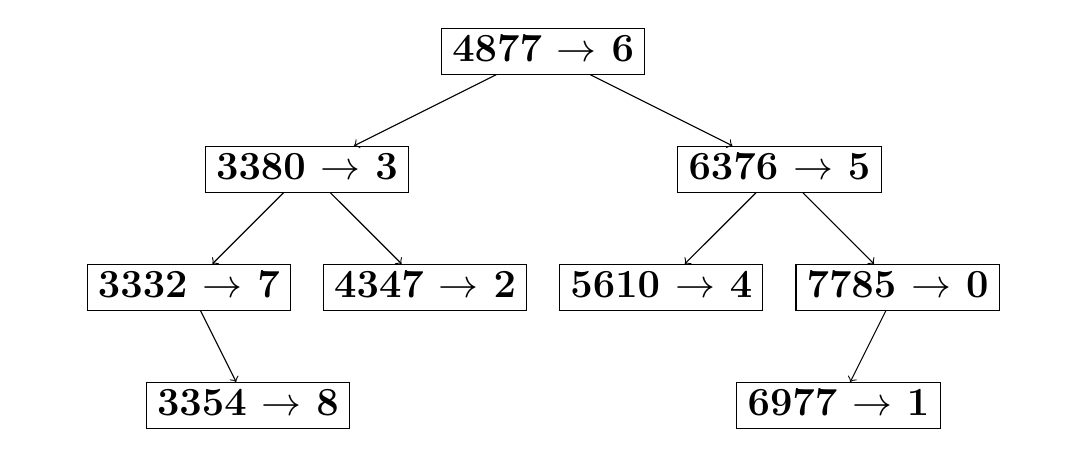
\begin{tikzpicture}
				\node[]								(4877)		[]		{\begin{tabular}{c}4877 $\rightarrow$ 6\end{tabular}}
					child[] {node[]						(3380)		[]		{\begin{tabular}{c}3380 $\rightarrow$ 3\end{tabular}}
 						child[] {node[]					(3332)		[]		{\begin{tabular}{c}3332 $\rightarrow$ 7\end{tabular}}
  							child[phantom node] {node[]	(phantom0)	[]		{\begin{tabular}{c}3354 $\rightarrow$ 8\end{tabular}}}
  							child[] {node[]				(3354)		[]		{\begin{tabular}{c}3354 $\rightarrow$ 8\end{tabular}}}}
						child[] {node[]					(4347)		[]		{\begin{tabular}{c}4347 $\rightarrow$ 2\end{tabular}}}}
					child[] {node[]						(6376)		[]		{\begin{tabular}{c}6376 $\rightarrow$ 5\end{tabular}}
 						child[] {node[]					(5610)		[]		{\begin{tabular}{c}5610 $\rightarrow$ 4\end{tabular}}}
 						child[] {node[]					(7785)		[]		{\begin{tabular}{c}7785 $\rightarrow$ 0\end{tabular}}
  							child[] {node[]				(6977)		[]		{\begin{tabular}{c}6977 $\rightarrow$ 1\end{tabular}}}
  							child[phantom node] {node[]	(phantom1)	[]		{\begin{tabular}{c}3354 $\rightarrow$ 8\end{tabular}}}}
				};
			
			\end{tikzpicture}
		\end{adjustbox}
		\vspace{-1.0em}
		\caption{A balanced search tree used to map page IDs to buffer frames.}
	\end{figure}}

\end{frame}

\begin{frame}[fragile]

	\frametitle{Hash Table}

	\begin{columns}
      		\column{.5\textwidth}
		
			\tikzset{%
				node distance = .5cm,
				bucketHeaderNumber/.style = {shape = rectangle, draw = black, minimum width = .2\textwidth, anchor = south west, minimum height = .5cm, font = \bfseries},
				bucketHeaderNext/.style = {shape = rectangle, draw = black, minimum width = .2\textwidth, anchor = south east, minimum height = .5cm},
				bucketBody/.style = {shape = rectangle split, rectangle split parts = #1, draw = black, minimum width = .4\textwidth, anchor = north},
				pid/.style = {draw = none, font = \bfseries},
				hashFunction/.style = {draw = black, shape = rectangle, rounded corners = 5pt, minimum height = 1.25\textheight, minimum width = .375\textwidth},
				hashFunctionText/.style = {font = \bfseries},
				hashFunction/.append style = {draw = ForestGreen, fill = ForestGreen!15}, 
				hashFunctionText/.append style = {text = ForestGreen},
				bucketHeaderNumber/.append style = {draw = Purple, fill = Purple!15},
				bucketHeaderNext/.append style = {draw = Purple!75, fill = Purple!11.25}
			}

			\centering
			\begin{adjustbox}{totalheight = \textheight - 4.0em}
				\uncover<2->{\begin{tikzpicture}
					
					% Create the hash function:
					\node[hashFunction]				(func)		[]						{};
					\node[hashFunctionText]			(funcText)		[below = .025cm of func.north]	{$\bm{\text{mod } 5}$};
					
					% Create the hashed Page IDs:
					\pgfmathsetseed{2144}
					\pgfmathsetmacro{\numOfPages}{4}
					\pgfmathsetmacro{\initialValue}{int(10000 * rand)}
					\ifthenelse{\initialValue < 0}{
						\pgfmathsetmacro{\initialValue}{int(-1 * \initialValue)}
					}{}
					\node[pid]							(pid0)		[left = of func]			{\initialValue};
					\node[]							(help0)		[right = of pid0]			{};
					\draw[]		(pid0.east)	--		(help0.west);
					\foreach \x in {1, ..., \numOfPages}{
						\ifthenelse{\x = 1}{
							\pgfmathtruncatemacro{\previousTop}{0}
							\pgfmathtruncatemacro{\previousBottom}{0}
						}{
							\pgfmathtruncatemacro{\previousTop}{(2 * \x) - 3}
							\pgfmathtruncatemacro{\previousBottom}{(2 * \x) - 2}
						}
						\pgfmathtruncatemacro{\top}{(2 * \x) - 1}
						\pgfmathtruncatemacro{\bottom}{(2 * \x)}
						\pgfmathsetmacro{\topValue}{int(10000 * rand)}
						\pgfmathsetmacro{\bottomValue}{int(10000 * rand)}
						\ifthenelse{\topValue < 0}{
							\pgfmathsetmacro{\topValue}{int(-1 * \topValue)}
						}{}
						\ifthenelse{\bottomValue < 0}{
							\pgfmathsetmacro{\bottomValue}{int(-1 * \bottomValue)}
						}{}
						
						\node[pid]							(pid\top)			[above = of pid\previousTop]			{\topValue};
						\node[]							(help\top)			[right = of pid\top]					{};
						\draw[]		(pid\top.east)	--		(help\top.west);
						\node[pid]							(pid\bottom)		[below = of pid\previousBottom]			{\bottomValue};
						\node[]							(help\bottom)		[right = of pid\bottom]				{};
						\draw[]		(pid\bottom)	--		(help\bottom);
					}
					
					% Create the hash buckets:
					\pgfmathsetmacro{\numOfBuckets}{2}
					\pgfmathsetmacro{\initialBucket}{int(\numOfBuckets)}
					\node[bucketBody=2]				(bucketBody2)		[right = of func, yshift = -.25cm]			{\nodepart{one}$4347 \rightarrow 2$\nodepart{two}$4877 \rightarrow 6$};
					\node[bucketBody=2]				(bucketBody1)		[above = 1cm of bucketBody2]			{\nodepart{one}$6376 \rightarrow 5$\nodepart{two}$\cdot$};
					\node[bucketBody=2]				(bucketBody3)		[below = 1cm of bucketBody2]			{\nodepart{one}$\cdot$\nodepart{two}$\cdot$};
					\node[bucketBody=2]				(bucketBody0)		[above = 1cm of bucketBody1]			{\nodepart{one}$3380 \rightarrow 3$\nodepart{two}$5610 \rightarrow 4$};
					\node[bucketBody=2]				(bucketBody4)		[below = 1cm of bucketBody3]			{\nodepart{one}$3354 \rightarrow 8$\nodepart{two}$\cdot$};
					\node[bucketHeaderNumber]		at (bucketBody0.north west)	(bucketHeaderNu0)	[]			{0};
					\node[bucketHeaderNext]			at (bucketBody0.north east)	(bucketHeaderNe0)	[]			{};
					\node[bucketHeaderNumber]		at (bucketBody1.north west)	(bucketHeaderNu1)	[]			{1};
					\node[bucketHeaderNext]			at (bucketBody1.north east)	(bucketHeaderNe1)	[]			{$\cdot$};
					\node[bucketHeaderNumber]		at (bucketBody2.north west)	(bucketHeaderNu2)	[]			{2};
					\node[bucketHeaderNext]			at (bucketBody2.north east)	(bucketHeaderNe2)	[]			{};
					\node[bucketHeaderNumber]		at (bucketBody3.north west)	(bucketHeaderNu3)	[]			{3};
					\node[bucketHeaderNext]			at (bucketBody3.north east)	(bucketHeaderNe3)	[]			{$\cdot$};
					\node[bucketHeaderNumber]		at (bucketBody4.north west)	(bucketHeaderNu4)	[]			{4};
					\node[bucketHeaderNext]			at (bucketBody4.north east)	(bucketHeaderNe4)	[]			{$\cdot$};
					\node[]							(bucketHelp0)		[left = of bucketHeaderNu0]			{};
					\node[]							(bucketHelp1)		[left = of bucketHeaderNu1]			{};
					\node[]							(bucketHelp2)		[left = of bucketHeaderNu2]			{};
					\node[]							(bucketHelp3)		[left = of bucketHeaderNu3]			{};
					\node[]							(bucketHelp4)		[left = of bucketHeaderNu4]			{};
					\draw[]		(bucketHeaderNu0.west)	--		(bucketHelp0.east);
					\draw[]		(bucketHeaderNu1.west)	--		(bucketHelp1.east);
					\draw[]		(bucketHeaderNu2.west)	--		(bucketHelp2.east);
					\draw[]		(bucketHeaderNu4.west)	--		(bucketHelp4.east);

					\node[bucketBody=4]				(bucketBody00)		[right = of bucketBody0, yshift = -.41cm]			{\nodepart{one}$7785 \rightarrow 0$\nodepart{two}$\cdot$\nodepart{three}$\cdot$\nodepart{four}$\cdot$};
					\node[bucketHeaderNumber]		at (bucketBody00.north west)	(bucketHeaderNu00)	[]			{0};
					\node[bucketHeaderNext]			at (bucketBody00.north east)	(bucketHeaderNe00)	[]			{$\cdot$};
					\draw[]		(bucketHeaderNe0.center)	--		(bucketHeaderNu00.west);

					\node[bucketBody=4]				(bucketBody20)		[right = of bucketBody2, yshift = -.445cm]			{\nodepart{one}$3332 \rightarrow 7$\nodepart{two}$6977 \rightarrow 1$\nodepart{three}$\cdot$\nodepart{four}$\cdot$};
					\node[bucketHeaderNumber]		at (bucketBody20.north west)	(bucketHeaderNu20)	[]			{2};
					\node[bucketHeaderNext]			at (bucketBody20.north east)	(bucketHeaderNe20)	[]			{$\cdot$};
					\draw[]		(bucketHeaderNe2.center)	--		(bucketHeaderNu20.west);

					\draw[]		(help5.west)	--		(bucketHelp0.east);
					\draw[]		(help1.west)	--		(bucketHelp0.east);
					\draw[]		(help8.west)	--		(bucketHelp0.east);
					\draw[]		(help4.west)	--		(bucketHelp1.east);
					\draw[]		(help7.west)	--		(bucketHelp2.east);
					\draw[]		(help3.west)	--		(bucketHelp2.east);
					\draw[]		(help0.west)	--		(bucketHelp2.east);
					\draw[]		(help6.west)	--		(bucketHelp2.east);
					\draw[]		(help2.west)	--		(bucketHelp4.east);
				\end{tikzpicture}}
			\end{adjustbox}
		
		\column{.5\textwidth}
			\begin{itemize}
				\uncover<3->{\item	Each page ID is mapped to a hash bucket using a hash function}
				\uncover<4->{\item	Only the page IDs of buffered pages are in the hash table}
				\uncover<5->{\item	If a hash bucket is full, a chained bucket gets added}
				\uncover<6->{\item	$T_{\text{avg}}^{\text{search}} \in  \mathcal O\left(1\right)$, \linebreak$T_{\text{avg}}^{\text{insert}} \in  \mathcal O\left(1\right)$, \linebreak$T_{\text{worst}}^{\text{search}} \in  \mathcal O\left(n\right)$}
			\end{itemize}
				
	\end{columns}

\end{frame}

\begin{frame}[fragile]

	\frametitle{Locate Pages in Buffer Pool with Hash Table \large(\cite{Graefe:2014})}
	
	\tikzset{%
		node distance = 1cm,
		startstop/.style = {rectangle, rounded corners, minimum width = 2cm, minimum height = 1cm, draw = red, fill = red!15, text width = 3cm, align = center},
		io/.style = {trapezium, trapezium left angle = 70, trapezium right angle = 110, minimum width = 2cm, minimum height = 1cm, draw = blue, fill = blue!15, text width = 2cm, align = center},
		process/.style = {rectangle, minimum width = 2cm, minimum height = 1cm, draw = orange, fill = orange!15, text width = 3cm, align = center},
		decision/.style = {diamond, aspect=2, minimum width = 2cm, minimum height = 1cm, draw = green, fill = green!15, text width = 3cm, align = center},
		arrow/.style = { -> , thick, >=stealth}
	}

	\noindent\makebox[\textwidth]{
		\begin{adjustbox}{width = \textwidth + 4.0em}
			\begin{tikzpicture}
				\node[visible on = <1->]							(center start)		[]						{};
				\node[visible on = <2->, io]						(page)			[left = of center start]			{Buffer pool page image};
				\node[visible on = <3->, io]						(key)				[right = of center start]		{Search key};
				\node[visible on = <4->, process]					(search)			[below = of center start]		{Look for entry in page image that corresponds to search key};
				\node[visible on = <5->, decision]					(found1)			[below = of search]			{Found entry?};
				\node[visible on = <6->, startstop]					(miss)			[below = of found1]			{Search key not found};
				\node[visible on = <7->, process]					(get id)			[right = of found1]			{Get identifier of the next page to search from the page image};
				\node[visible on = <8->, process]					(hash)			[below = of get id]			{calculate hash id of the page id};
				\node[visible on = <9->, process]					(lookup)			[right = 1.5cm of hash]		{Look in buffer pool hash table for hashed page id (protect hash table)};
				\node[visible on = <10->, decision]					(found2)			[above = of lookup]			{Found hashed page id?};
				\node[visible on = <12->, process]					(load)			[above = of found2]			{Bring page into buffer pool (possibly need to evict another page image)};
				\node[visible on = <11->, startstop]					(final)			[right = of found2]			{Return buffer pool page image of the next page to search};

				\draw[visible on = <4->, arrow]	(page)			-|						(search);
				\draw[visible on = <4->, arrow]	(key)				-|						(search);
				\draw[visible on = <5->, arrow]	(search)			--						(found1);
				\draw[visible on = <6->, arrow]	(found1)			--	node[right]	{no}		(miss);
				\draw[visible on = <7->, arrow]	(found1)			--	node[above]	{yes}		(get id);
				\draw[visible on = <8->, arrow]	(get id)			--						(hash);
				\draw[visible on = <9->, arrow]	(hash)			--						(lookup);
				\draw[visible on = <10->, arrow]	(lookup)			--						(found2);
				\draw[visible on = <12->, arrow]	(found2)			--	node[right]	{no}		(load);
				\draw[visible on = <11->, arrow]	(found2)			--	node[above]	{yes}		(final);
				\draw[visible on = <13->, arrow]	(load)			-|						(final);
			\end{tikzpicture}
		\end{adjustbox}
	}

\end{frame}

\subsection{Locate Pages in the Buffer Pool with Pointer Swizzling}

\frame{\subsectionpage}

\begin{frame}

	\frametitle{Pointer Swizzling}
	
	\begin{block}{Definition}
		\justify
		To swizzle a pointer means to transform the address of the persistent object referenced there to a more direct address of the transient object in a way that this transformation could be used during multiple indirections of this pointer (\cite{Moss:1992}).
	\end{block}
	
\end{frame}

\begin{frame}[fragile]

	\frametitle{Classification of the Pointer Swizzling Approach following \cite{White:1995}}

	\tikzset{%
		selected/.style = {font = \bfseries, very thick},
		selected/.append style = {text = blue, color = blue}
	}

	\vspace{-1.5em}
	\centering
	\begin{adjustbox}{totalheight = \textheight - 2.0em}
		\begin{tikzpicture}
			\draw arc [start angle = 0,   
                 				end angle = 360,
                					x radius = 4cm, 
                 				y radius = 4cm]
						node [visible on = <5->, pos = 1 * 1/14]				(eager)		{eager}
						node [visible on = <6->, pos = 2 * 1/14, selected]		(direct)		{direct}
						node [visible on = <7->, pos = 3 * 1/14, selected]		(in-place)		{in-place}
						node [visible on = <3->, pos = 4 * 1/14]				(hardware)	{hardware}
						node [visible on = <2->, pos = 5 * 1/14]				(no-swizzling)	{no-swizzling}
						node [visible on = <8->, pos = 6 * 1/14]				(no uncaching)	{no uncaching}
						node [visible on = <4->, pos = 7 * 1/14]				(partial)		{partial}
						node [visible on = <5->, pos = 8 * 1/14, selected]		(lazy)		{lazy}
						node [visible on = <6->, pos = 9 * 1/14]				(indirect)		{indirect}
						node [visible on = <7->, pos = 10 * 1/14]				(copy)		{copy}
						node [visible on = <3->, pos = 11 * 1/14, selected]		(software)		{software}
						node [visible on = <2->, pos = 12 * 1/14, selected]		(swizzling)		{swizzling}
						node [visible on = <8->, pos = 13 * 1/14, selected]		(uncaching)	{uncaching}
						node [visible on = <4->, pos = 14 * 1/14, selected]		(full)			{full};
			
			\node[anchor = center, right = 4cm of partial.center]			(center)			{};
			\path[->]	
				(center.center)		edge[visible on = <6->, selected]	(direct)
				(center.center)		edge[visible on = <6->]			(indirect)
				(center.center)		edge[visible on = <7->, selected]	(in-place)
				(center.center)		edge[visible on = <7->]			(copy)
				(center.center)		edge[visible on = <3->]			(hardware)
				(center.center)		edge[visible on = <3->, selected]	(software)
				(center.center)		edge[visible on = <4->]			(partial)
				(center.center)		edge[visible on = <4->, selected]	(full)
				(center.center)		edge[visible on = <2->]			(no-swizzling)
				(center.center)		edge[visible on = <2->, selected]	(swizzling)
				(center.center)		edge[visible on = <5->]			(eager)
				(center.center)		edge[visible on = <5->, selected]	(lazy)
				(center.center)		edge[visible on = <8->]			(no uncaching)
				(center.center)		edge[visible on = <8->, selected]	(uncaching);
		\end{tikzpicture}
	\end{adjustbox}

\end{frame}

\begin{frame}[fragile]

	\frametitle{Locate Pages in Buffer Pool w/ Pointer Swizzling \large(\cite{Graefe:2014})}

	\tikzset{%
		node distance = 1cm,
		startstop/.style = {rectangle, rounded corners, minimum width = 3cm, minimum height = 1cm,text centered, draw = red, fill = red!15},
		io/.style = {trapezium, trapezium left angle = 70, trapezium right angle = 110, minimum width = 3cm, minimum height = 1cm, text centered, draw = blue, fill = blue!15},
		process/.style = {rectangle, minimum width = 3cm, minimum height = 1cm, text centered, draw = orange, fill = orange!15},
		decision/.style = {diamond, minimum width = 3cm, minimum height = 1cm, text centered, draw = green, fill = green!15},
		arrow/.style = { -> , thick, >=stealth}
	}

	\noindent\makebox[\textwidth]{
		\begin{adjustbox}{width = \textwidth + 4.0em}
			\begin{tikzpicture}
				\node[visible on = <1->]							(center start)		[]						{};
				\node[visible on = <2->, io]						(page)			[left = of center start]			{\begin{tabular}{c}Buffer pool\\page image\end{tabular}};
				\node[visible on = <3->, io]						(key)				[right = of center start]		{Search key};
				\node[visible on = <4->, process]					(search)			[below = of center start]		{\begin{tabular}{c}Look for entry\\in page image\\that corresponds\\to search key\end{tabular}};
				\node[visible on = <5->, decision]					(found)			[below = of search]			{\begin{tabular}{c}Found\\entry?\end{tabular}};
				\node[visible on = <6->, startstop]					(miss)			[below = of found]			{\begin{tabular}{c}Search key\\not found\end{tabular}};
				\node[visible on = <7->, process]					(get id)			[right = of found]			{\begin{tabular}{c}Get identifier of\\the next page\\to search from\\the page image\end{tabular}};
				\node[visible on = <8->, decision]					(swizzled)			[right = of get id]			{\begin{tabular}{c}Identifier\\swizzled?\end{tabular}};
				\node[visible on = <10->, process]					(load)			[above = of swizzled]			{\begin{tabular}{c}Bring page into\\buffer pool (possibly\\need to evict another\\ page image) and\\swizzle pointer on it\end{tabular}};
				\node[visible on = <9->, startstop]					(final)			[right = of swizzled]			{\begin{tabular}{c}Return buffer pool\\page image of the next\\page to search\end{tabular}};

				\draw[visible on = <4->, arrow]	(page)			-|						(search);
				\draw[visible on = <4->, arrow]	(key)				-|						(search);
				\draw[visible on = <5->, arrow]	(search)			--						(found);
				\draw[visible on = <6->, arrow]	(found)			--	node[right]	{no}		(miss);
				\draw[visible on = <7->, arrow]	(found)			--	node[above]	{yes}		(get id);
				\draw[visible on = <8->, arrow]	(get id)			--						(swizzled);
				\draw[visible on = <10->, arrow]	(swizzled)			--	node[right]	{no}		(load);
				\draw[visible on = <9->, arrow]	(swizzled)			--	node[above]	{yes}		(final);
				\draw[visible on = <11->, arrow]	(load)			-|						(final);
			\end{tikzpicture}
		\end{adjustbox}
	}

\end{frame}
